\section{Introduction}
The synthesis of doped barium zirconate in bulk configurations is an important component of this research. Bulk samples derived from precursor powders have strong appeal from an applications point of view because of their relative ease of production. Powder-based bulk barium zirconate that could be effective as an electrolyte in fuel cell systems are desirable. These samples also allow experimentation with sintering parameters, bench marking of basic crystallographic characteristics, and measurements of the electrical properties of polycrystals. Moreover, bulk samples can be used as the laser ablation targets necessary for the PLD process of thin film deposition. For all these reasons, it is essential to synthesize and characterize bulk specimens. Bulk samples used in this project were produced by essentially two different approaches:  (1) Solid state reaction of barium carbonate, zirconium oxide and dopant oxide, and (2) Chemical solution techniques based on carbohydrates and metal salts. XRD was selectively used for monitoring chemical reactions through the synthesis, when applicable, and allowed the observation of changes in the diffraction patterns. In some cases XRD also enabled the determination of the lattice parameters of the underlying crystal and the effect of different dopants and concentrations. 

%(1) Mixture and thermal treatment of an oxide containing the dopant with stoichiometric barium zirconate powder;

%Comparisons of these changes show the effects of dopant ionic radius on the unit cell structure. 
%We investigate the synthesis of the targets and compare their structural properties to those of the thin films. The targets serve as precursor material to the thin films and as such their composition and structure serve as a baseline of comparison. 

%To characterize thin films, XRD is employed in order to discern crystalline versus amorphous structure as well calculate lattice parameters. The structure of the films vary with the deposition temperature and comparing the relative intensity of peaks shows the increase in crystallographic structure. In addition to structure, the thickness of these films was investigated with spectrophotometry, comparing the thin film interference of different wavelengths of light. By using difference incident angles, the index of refraction for this material was calculated. 

\vspace{12pt}
\section{Synthesis and structural characterization of bulk samples}

%\section{Target and Pellet synthesis and preparation}
%This section probably belongs in the section on pellet conductivity. Although this could be a section devoted to synthesis and methods of all kinds? Pellets, thin films, and contacts?
%An introduction here outlining the methods to produce the targets and maybe the qualities of a good target.
%\subsection{Directly Sintered Powders - poor stoichiometry}
%direct mixing and sintering
%adding extra bco to aid stoichiometry
%results?

\subsection{Solid State Reaction}

The most straightforward method of synthesis for barium zirconate involves a solid state chemical reaction between barium carbonate and zirconium oxide. For meaningful rates, this well known reaction requires temperatures in excess of 1100$^\circ$C. Adapting this reaction for obtaining  doped barium zirconate can be accomplished by the addition of an oxide of the dopant element in the desired amount. The reaction can be summarized in the following equation where M stands for the dopant element, which in our studies was Y, Yb, or Gd:
%falls under the classification of [some kind of archetype] and 
% (??) and compensating for this stoichiometry with the appropriate addition of barium zirconate
\begin{equation}
    \mathrm{BaCO_3 + \text{\ensuremath{x}}ZrO_2 + \left(\frac{1-\it{x}}{2}\right) M_2 O_3 \longrightarrow BaZr_\text{\ensuremath{x}} M_{1-\text{\ensuremath{x}}}O_{3-\delta} + CO_2}.
    \label{meth:equ:ssr}
\end{equation}

\begin{figure}
    \centering
    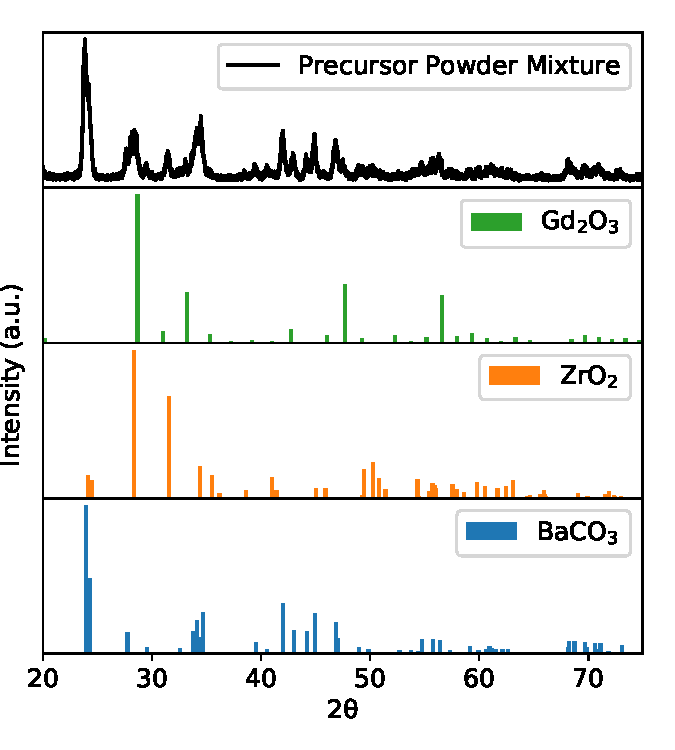
\includegraphics{Figures/170606-xrd-ssr-reaction-monitoring-before-rxn-separate-plots.pdf}
    \caption{X-ray diffraction pattern measured from a pressed pellet of as-mixed precursor powders prior to heat treatment. Standard patterns from each of the constituent powders are shown for reference.}
    \label{fig:target:xrd:reaction:before:separated}
\end{figure}

A complication in the implementation of the reaction of equation \ref{meth:equ:ssr} is the tendency for barium to be lost at high temperatures. The shift in stoichiometry caused by barium loss drives the dopant element into the A-site of the perovskite structure, which is highly detrimental to the ionic conductivity of the resulting material. Barium loss can be compensated for by adding an excess of $\sim$10\% barium carbonate to the process. Accordingly, all samples produced by solid state reaction in the subsequent studies were synthesized with 10\% by weight excess barium carbonate. 



The reagents used in the reaction of equation \ref{meth:equ:ssr} were in the form of precursor powders. They were mixed with mortar and pestle and pressed at 2800 psi. Figure \ref{fig:target:xrd:reaction:before:separated} shows a typical XRD pattern of the precursor powder mixture as measured prior to any heat treatment and compared with reference patterns for each of the compounds included in the mixture. The reaction proceeded by heat treatments at temperatures in the 1300-1600$^\circ$C range in air for times between 5 and 32 hours. Heat-treated samples were then analyzed by XRD to assess the degree of precursor phase change and formation of the intended barium zirconate phase.
%We carried out the solid state reaction both without and with the inclusion of excess barium carbonate as discussed. 

The reaction caused a volume change in the pellets that led to cracks and loss of mechanical integrity. This required crushing, re-mixing with mortar and pestle, and re-pressing at the same 2800 psi pressure. Figure \ref{fig:target:xrd:reaction:bzgxs10} shows a typical series of XRD patterns measured through the thermal history of the production of a bulk sample, in which the dopant used was Gd at a doping level of 10 mol\%.  
\begin{figure}
    \centering
    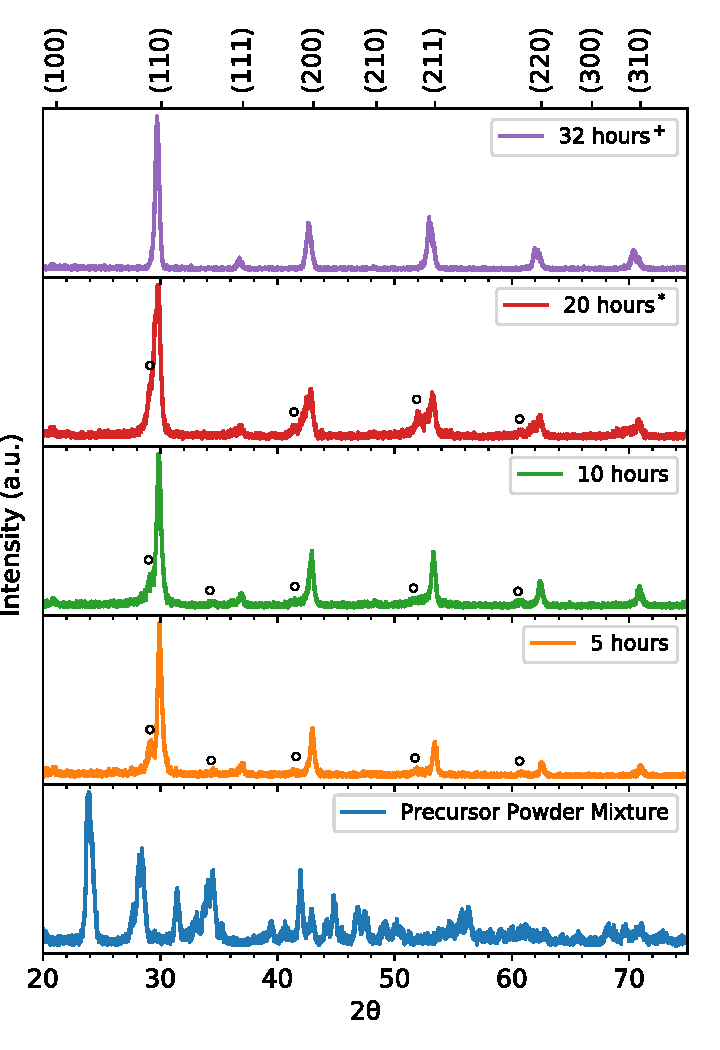
\includegraphics{Figures/170629-xrd-BZGxs10-reaction-monitor-2-edit-3.pdf}
    \caption{X-ray diffraction patterns of a bulk sample of barium zirconate with intended doping with 10 mol\% Gd. Each pattern was taken after completion of a significant thermal processing step as shown in the figure legend. Thermal processing during the initial 10 hours took place at 1300\textdegree C. Thermal processing steps marked by an asterisk (*) and plus (+) were carried out at elevated temperature of 1550\textdegree C and 1600\textdegree C, respectively. Peaks marked with a circle ($\circ$) represent BaGd$_2$O$_4$ reflections.}
    \label{fig:target:xrd:reaction:bzgxs10}
\end{figure}

The rationale of the temperature treatment seen in Figure \ref{fig:target:xrd:reaction:bzgxs10} is guided by the barium zirconate literature and our own experience in the processing of this high temperature ceramic. The initial steps at 1300\textdegree C are meant to sufficiently drive the solid state reaction while attempting to limit the loss of barium and the volume change of the pellet. As dopant incorporation increases and the material becomes more homogeneous, higher temperatures are used to initiate the sintering of the grains. After a total processing time of 32 hours, at the increasing temperature stages of 1300\textdegree C (10 hrs), 1550\textdegree C (10 hrs), and 1600\textdegree C (12 hrs), one can ascertain from the XRD pattern that the reaction is complete. The final step at 1600\textdegree C takes place in an alumina crucible with an excess of sacrificial mixture of barium zirconate and barium carbonate powder surrounding the sample on all sides to prevent barium loss.


One final processing step of the sintered bulk samples involved the polishing with 400 grit silicon carbide paper to improve surface uniformity. This step enhances electrical contact performance in preparation for EIS measurements and also improves reproducibility of thin film deposition when the bulk samples are used as laser ablation targets in the PLD thin film fabrication process. 

%We found that one calcination step reaction was sufficient to complete the reaction leading to single phase barium zirconate. Further calcination and crushing and pressing steps resulted in no change to the XRD pattern as shown in Figure \ref{fig:target:xrd:reaction:after}.
%and mounted in the PLD chamber using silver glue. 
%\begin{figure}
%    \centering
%    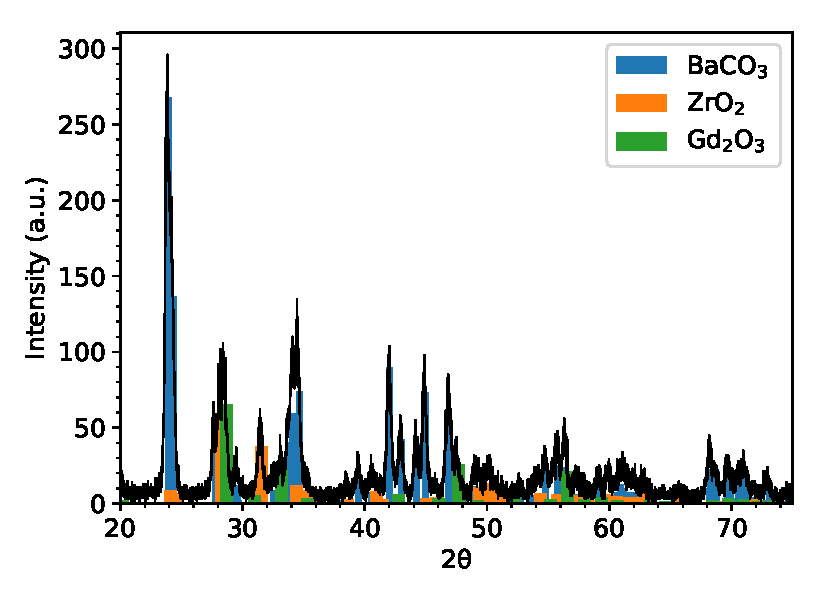
\includegraphics{Figures/170606-xrd-ssr-reaction-monitoring-before-rxn.pdf}
%    \caption{X-ray diffraction pattern of powder precursor mixture prior to solid state reaction.}
%    \label{fig:target:xrd:reaction:before}
%\end{figure}
%After the reaction step at 1300\textdegree C, the pellet was crushed and repressed and an XRD pattern was 
%\begin{figure}
%    \centering
%    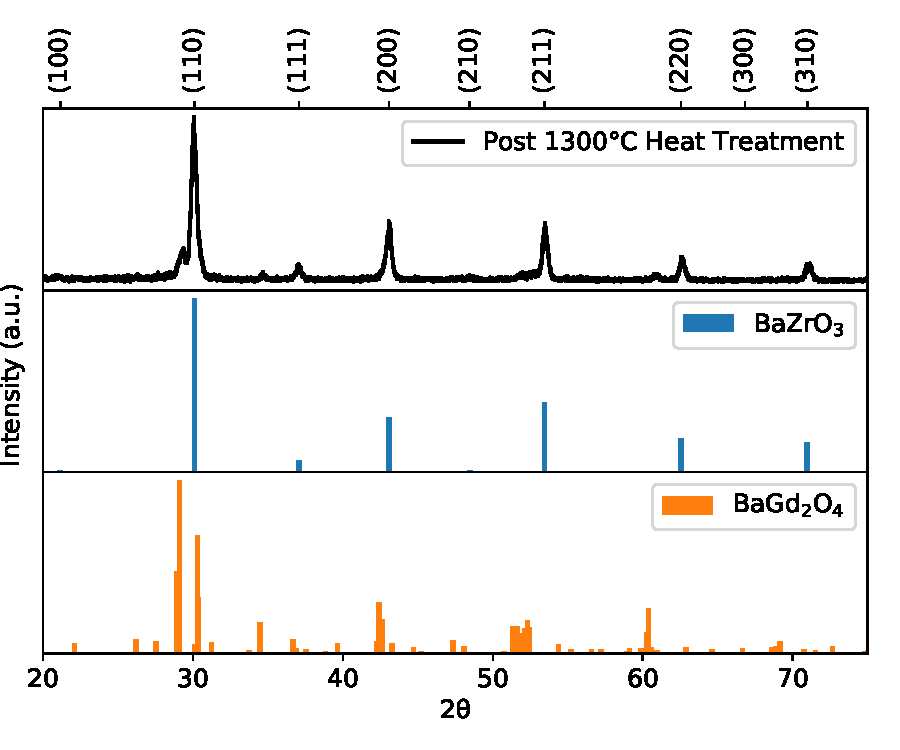
\includegraphics{Figures/170606-xrd-ssr-reaction-monitoring-after-rxn-separate-plots.pdf}
%    \caption{Following calcination at 1300\textdegree C for 5 hours.}
%    \label{fig:target:xrd:reaction:after}
%\end{figure}

%\begin{figure}
%    \centering
%    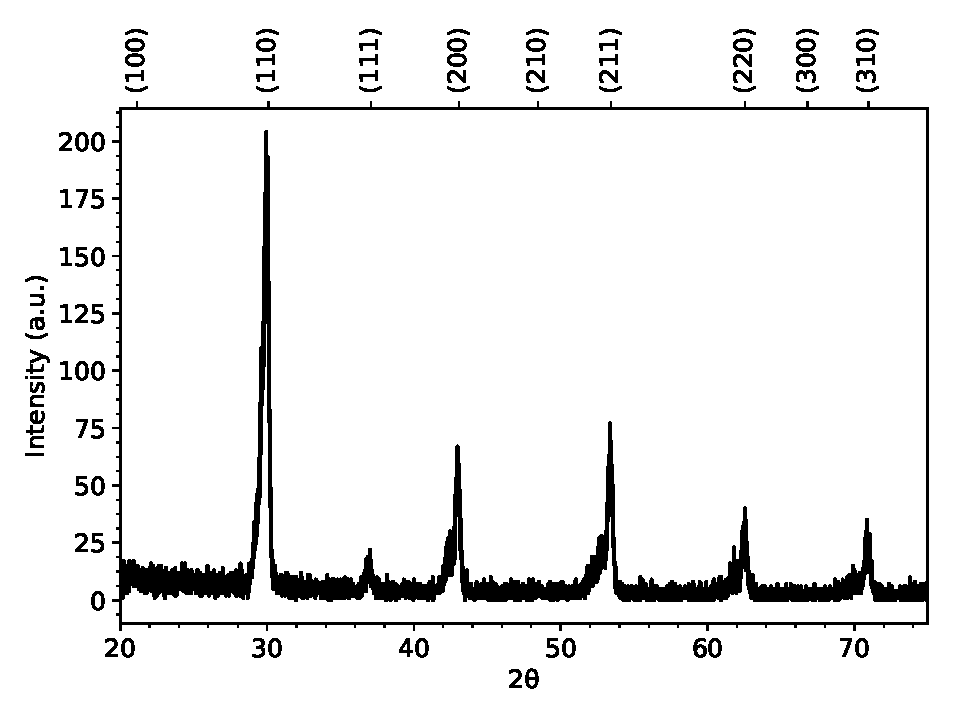
\includegraphics[width=\linewidth]{Figures/170606-xrd-ssr-reaction-monitoring-after-sinter-test.pdf}
%    \caption{After sintering at 1550\textdegree C for 5 hours}
%    \label{fig:target:xrd:reaction:sinter}
%\end{figure}
%We repeated the solid state reaction and sintering  protocols described above with the addition of 10\% by weight excess barium carbonate, in order to compensate for any loss of barium oxide during the reaction.
%We then followed this calcification step with a sintering step in order to obtain a pellet that was dense and hard enough to serve as a suitable target in the PLD process. Fig \ref{fig:target:xrd:reaction:sinter} shows the results of this sintering along with the peak indices of barium zirconate. 

\vspace{12pt}
\subsection{Chemical Solution Techniques}
Chemical solution methods offer advantages of better mixing of molecules to provide a more homogeneous precursor powder, as well as lower reaction temperature and reaction time, preventing unwanted barium loss and thus enhancing the potential for proper stoichiometry. Many variations of chemical approaches have been discussed in the literature. In essence, virtually all of them combine metal salts as precursors for the ultimate ceramic constituents, and hydrocarbons that serve to bind the various metal ions in a well-dispersed solution. After homogenized, the solution is subject to one or more combustion reactions that lead to the carbonization of the organic phase, leaving behind a well-mixed stoichiometric inorganic phase that can be further processed for sintering purposes, as needed. 

Most solution techniques derive their main characteristics from the traditional Pechini method \cite{Pechini1967}. This approach involves mixing of metal nitrate salts with ethylenediaminetetraacetic acid (EDTA) and/or citric acid and ethylene glycol to form a metal ion aqueous mixture that undergoes a polymerization reaction to form a resin after heating for several hours at 80\textdegree C. Further heating chars the resin, which can then be calcinated at 900\textdegree C for further oxidation of the resin and crystallization of the inorganic species. Modifications of the Pechini method have been reported by several authors. A common variation involves a rapid reaction and high temperatures as metal nitrate salts are mixed with either glycine \cite{Chick1990} or citric acid \cite{Gilardi2017}. The nitrates act as oxidizers and glycine/citric acid serves to bind to the various metal ions to provide a close mixing prior to the combustion reaction as well as serve as the fuel. In the case of gadolinium-doped barium zirconate, this can be accomplished by mixing desired molar ratios of the starting materials of Ba(NO$_3$)$_2$, Gd(NO$_3$)$_2$, and ZrO(NO$_3$)$_2 \cdot$ $x$H$_2$O (degree of hydration $x$ varies and can be determined through thermogavimetric analysis \cite{Babilo2007b}). The aqueous solution is dehydrated over a period of hours and increases in viscosity until a gel is formed, which autoignites to produce a powder ash. This powder can be calcinated at 1200-1300\textdegree C for several hours to produce a single-phase powder. 

\begin{figure}
    \centering
    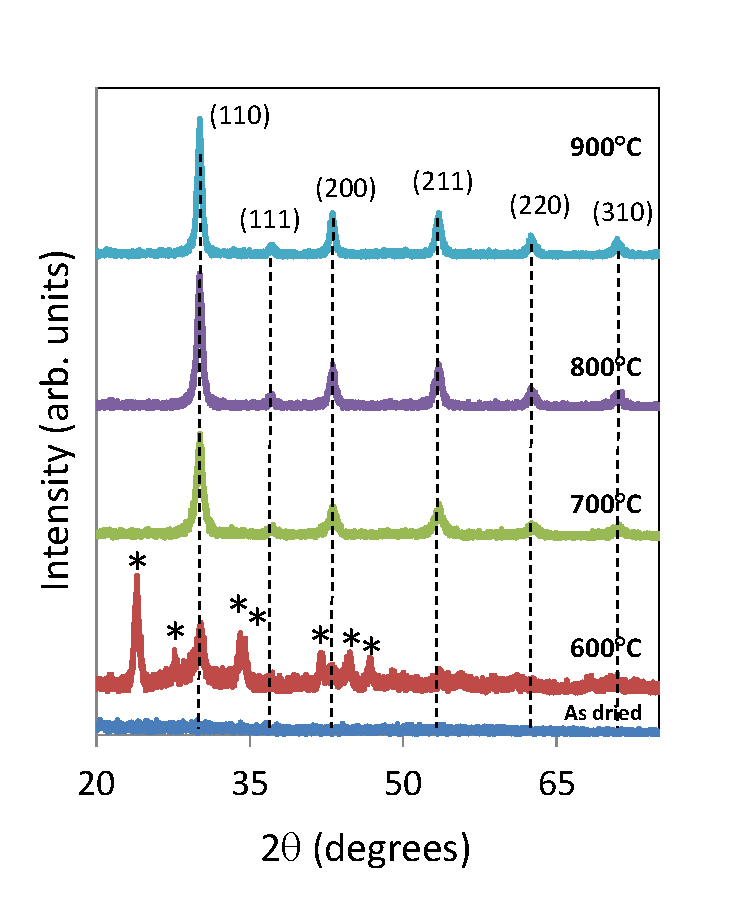
\includegraphics[scale=.8]{Figures/XRD_UAB_Chemical_Method.pdf}
    \caption{X-ray diffraction patterns of as-dried and temperature-treated 15\% Gd-doped BaZrO$_3$ samples at various temperatures. The indexed peaks (Miller indices) correspond to the cubic BaZrO$_3$ structure. The peaks indicated by asterisks most likely correspond to reflections of a barium compound, other than BaZrO$_3$, present prior to complete organic elimination that occurred between 600\textdegree C and 700\textdegree C. Reproduced from Ref. \cite{GCamata2015} with permission.}
    \label{fig:XRD:UAB:Chemical}
\end{figure}

In our research group we have explored a similar approach with slightly different precursors. Barium nitrate, zirconium tetraisopropoxide, citric acid, and ethylene glycol were employed, with the addition of gadolinium nitrate as the dopant source. With guidance from colleagues at the UAB Department of Chemistry and technical assistance of a local high school student, a procedure based on the literature was cautiously followed to generate a BaZrO$_3$ powder nominally doped with Gd. The details of the procedure are provided in Appendix C. The main result is shown in Figure \ref{fig:XRD:UAB:Chemical}, which displays X-ray diffraction patterns of the chemically-prepared compound in various stages of the synthesis, including the as-dried substance, which had the properties of a resin, as well as patterns measured after the compound was heat-treated in air at temperatures between 600\textdegree C and 900\textdegree C. 

As seen in Figure \ref{fig:XRD:UAB:Chemical}, the as-dried sample showed no distinguishable peaks, indicating the amorphous nature of the resin prior to heat treatment. After high-temperature treatments in air, the peaks of BaZrO$_3$ are clearly present at temperatures as low as 600\textdegree C. However, as shown by asterisks, peaks from another compound dominate the sample treated at 600\textdegree C. These other peaks may be due to other barium-based compounds, such as barium oxalate. Upon annealing at 700\textdegree C, all non-BaZrO$_3$ reflections are removed. The XRD patterns appear unchanged between 700\textdegree C and 900\textdegree C, with only BaZrO$_3$ peaks remaining in the samples. The processing temperature of 700\textdegree C required to obtain single-phase BaZrO$_3$ is significantly lower than temperatures required for Gd-doped BaZrO$_3$ synthesis based on the solid state reaction approach of equation \ref{meth:equ:ssr} discussed in the previous section. Chemical methods are therefore promising in avoiding barium loss and creating bulk materials with appropriate atomic scale incorporation of dopants at the proper zirconium site.

Although potentially effective as a bulk material, the powder yield of the process described in Appendix C proved to be low and the amount of powder produced in-house by the procedure was unsuitable for pressing the needed pellets. The costs involved in the large amounts of chemical precursors needed and the time-consuming effort to synthesize the tens of grams required for robust bulk samples were impractical. 

Another variation of the Pechini method performs the combustion step on atomized portions of the well-mixed chemical precursors, after it being sprayed. This approach further overcomes inhomegeneity issues by achieving the mixing of metal ions essentially on a molecular scale. First, a stoichiometric solution of metal salts is again prepared and a carbohydrate is added. The solution is then atomized into fine droplets which are dehydrated in a hot spray dryer chamber. As the droplets are dehydrated, they decrease in size and reach a critical concentration. By applying additional thermal energy, an explosive exothermic reaction is initiated. This reaction generates enough heat to rapidly convert the metal salts to their respective oxides and/or carbonates while maintaining the microscale mixing \cite{Praxair2019}. As a result, the precursor powder is comprised of individual particles which are homogeneous and stoichiometrically correct mixtures. Because of the more complex chemical spray technology involved, it was more effective to contract with an external vendor to have this type of bulk sample produced \cite{Praxair2019}. Figure \ref{fig:CSP} illustrates this approach, which is known as combustion spray pyrolysis. 

%Using the CSP process, Praxair is capable of producing powders with surface areas ranging from 2m2 / g to > 100m2 / g and particle size as fine as lOOnm (varies with chemistry). To date, the versatility of the CSP process has facilitated its application in over 600 different formulations.

%PSC uses a ceramic powder manufacturing process which overcomes many of the drawbacks of traditional powder processing. By incorporating solution techniques, PSC is able to mix metal ions on a molecular scale. First, a stoichiometric solution of metal salts is prepared and a carbohydrate is added. The solution is then atomized into fine droplets which are dehydrated in a hot spray dryer chamber. As the droplets are dehydrated, they decrease in size and reach a critical concentration. By applying additional thermal energy. an explosive exothermic reaction is initiated. This reaction generates enough heat to instantaneously convert the metal salts to their respective oxides and/ or carbonates while maintaining the microscale mixing. As a result, the precursor powder is comprised of individual particles which are homogeneous and stoichiometrically correct mixtures. Using the CSP process, Praxair is capable of producing powders with surface areas ranging from 2m2 / g to > 100m2 / g and particle size as fine as lOOnm (varies with chemistry). To date, the versatility of the CSP process has facilitated its application in over 600 different formulations.

\begin{figure}
    \centering
    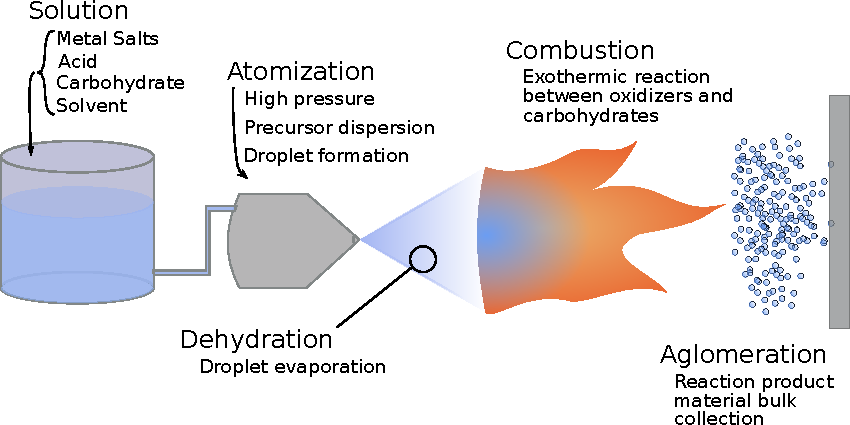
\includegraphics{Figures/Combustion_Spray_Pyrolysis-2.pdf}
    \caption{Outline of process used to produce Gd-doped bulk samples by combustion spray pyrolysis \cite{Praxair2019}.}
    \label{fig:CSP}
\end{figure}

Figure \ref{fig:target:xrd:praxbzg} shows a 2$\theta$ XRD scan of the a gadolinium-doped barium zirconate produced by combustion spray pyrolysis after sintering. The pattern confirms a high-quality, single-phase material with well-defined peaks for all BaZrO$_3$ reflections. Very small residual peaks for the precursor BaCO$_3$ are noted. A small amount of BaCO$_3$ residue is a common occurrence in BaZrO$_3$ synthesis throughout the literature and is generally not considered to be of significant consequence. The BaZrO$_3$ lattice parameter determined from this chemical spray pyrolysis target, was 4.221 \AA, similar to values obtained from bulk samples produced by solid state reaction.  
\begin{figure}
    \centering
    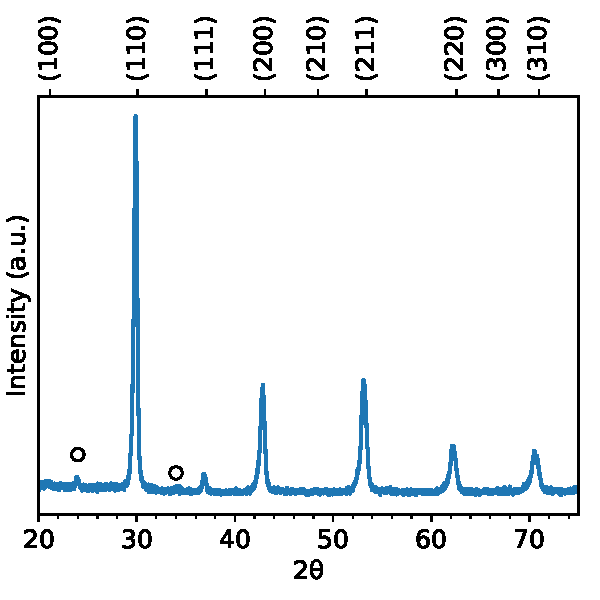
\includegraphics{Figures/181115-xrd-PraxBZG-pellet.pdf}
    \caption{2$\theta$ XRD scan of bulk sample of sintered gadolinium-doped barium zirconate produced by combustion spray pyrolysis; The circles ($\circ$) indicate reflections of residual BaCO$_3$ precursor material.}
    \label{fig:target:xrd:praxbzg}
\end{figure}

\vspace{12pt}
\section{Assessing Structural Effects as a Function of Dopant Incorporation}

Because of their different atomic radii, different dopants are expected to lead to distinct values of lattice parameter in the host BaZrO$_3$ lattice. Accordingly, we evaluated this possible effect by carrying out the solid state reaction synthesis of doped BaZrO$_3$ with the intended dopants Gd, Y, and Yb. We also analyzed the undoped bulked material. The 2$\theta$ XRD patterns after the reaction step at 1300\textdegree C of bulk samples produced with these various dopants can be seen in Figure \ref{fig:target:xrd:reaction:dopants}. Following the higher 1600\textdegree C temperature processing step the results can be seen in Figure \ref{fig:target:xrd:allTargetComparison}. 

\begin{figure}
    \centering
    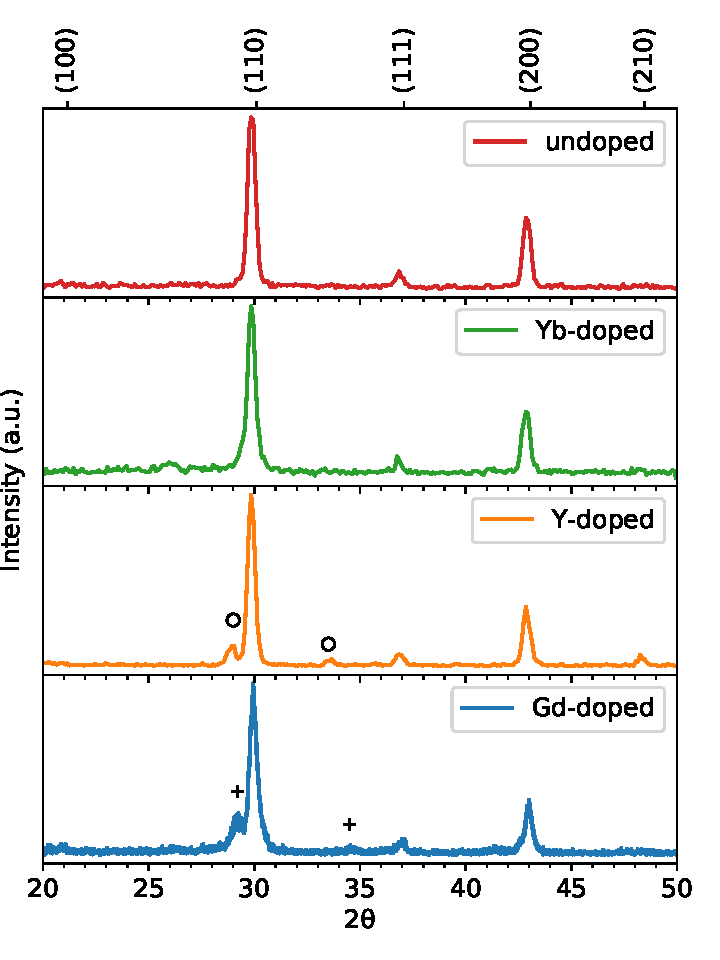
\includegraphics{Figures/xrd-pellet-dopant-comparison.pdf}
    \caption{Comparison of targets with different dopants following the reaction process at 1300\textdegree C for 5 hours. ($\circ$) and (+) mark BaY$_2$O$_4$ and BaGd$_2$O$_4$ reflections, respectively.}
    \label{fig:target:xrd:reaction:dopants}
\end{figure}

\begin{figure}
    \centering
    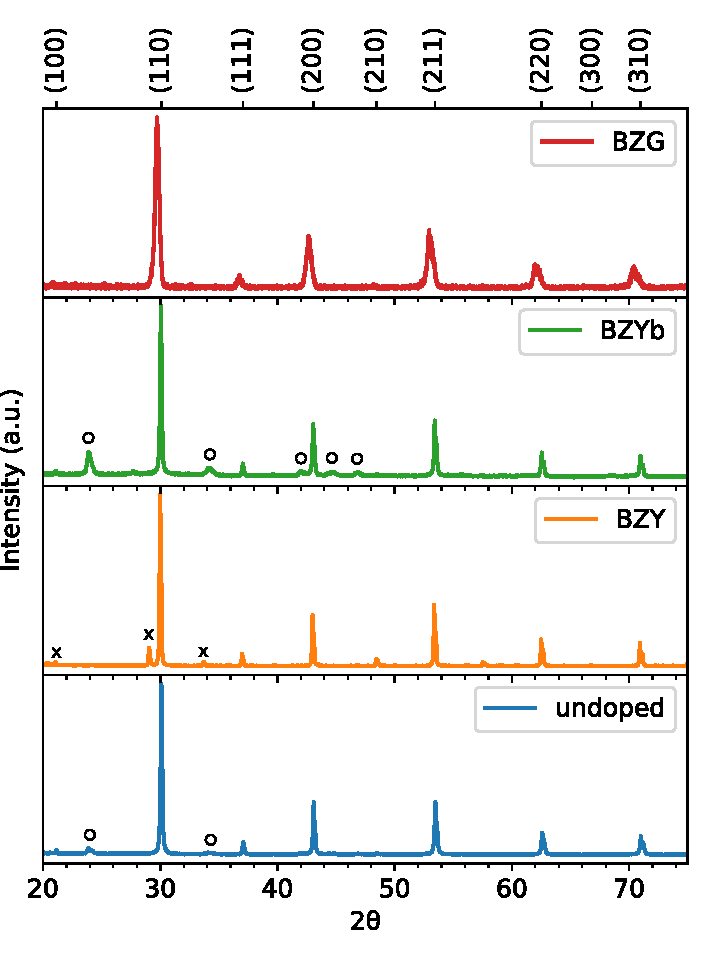
\includegraphics{Figures/190219-xrd-pure-y-yb-gd-pellet-comparison-edit-2.pdf}
    \caption{XRD of targets made with different dopants following 1600\textdegree C heat treatment. Peaks marked with a circle ($\circ$) are BaCO$_3$. Peaks marked with (x) are BaY$_2$O$_4$.}
    \label{fig:target:xrd:allTargetComparison}
\end{figure}

An interesting transitional stage of the material doped with gadolinium can be observed in Figure \ref{fig:target:xrd:reaction:dopants}. After the initial heat treatment step at 1300\textdegree C for 5 hours, a prominent reflection at $2\theta \approx$ 29\textdegree$\,$  is noted. This diffraction peak is identified as the (032) reflection of BaGd$_2$O$_4$. This is evidence that the presence of excess barium in the reaction is effective. This reaction step led to formation of a secondary phase in which the dopant (Gd in this case) occupies the B-site of the perovskite structure, which is exactly what is intended for achieving a controlled concentration of oxygen vacancies. Again, the excess barium is meant to prevent A-site incorporation and desorption of barium oxide. Subsequent heat treatment steps show that the peaks associated with BaGd$_2$O$_4$ disappear, likely indicating the incorporation of the dopant in the desired site of the cubic perovskite structure as barium continued to be lost.

To validate this idea of dopant incorporation in these heating processes, and analysis of the change in lattice parameters of the crystalline structure was undertaken. To calculate lattice parameters from an XRD pattern following the method of De Graef \cite{DeGraef2007}, the peak location, $\theta$ is used in the well known Bragg's Law formula for constructive interference $$2 d \sin{\theta} = n \lambda$$
along with the relation between the interplanar distance $d$ in a cubic system and the lattice spacing $a$ $$d = \frac{a}{\sqrt{h^2+k^2+l^2}}$$ Combining these two expressions give 
\begin{equation}
    a = \frac{\lambda \sqrt{h^2+k^2+l^2}}{2 \sin{\theta}}
    \label{xrd:latticeParameter}
\end{equation}
Using this equation we can write down a lattice parameter obtained from each diffraction angle. In order to fit the data and extract peak location, a best fit was established using a minimization routine employing Pseudo-Voigt profiles. An example of this fitting can be seen in Figure \ref{fig:target:xrd:fitComparison}, where in this case the $K\alpha1$ and $K\alpha2$ peaks can be resolved and fit with two Pseudo-Voigt profiles. 

\begin{figure}
    \centering
    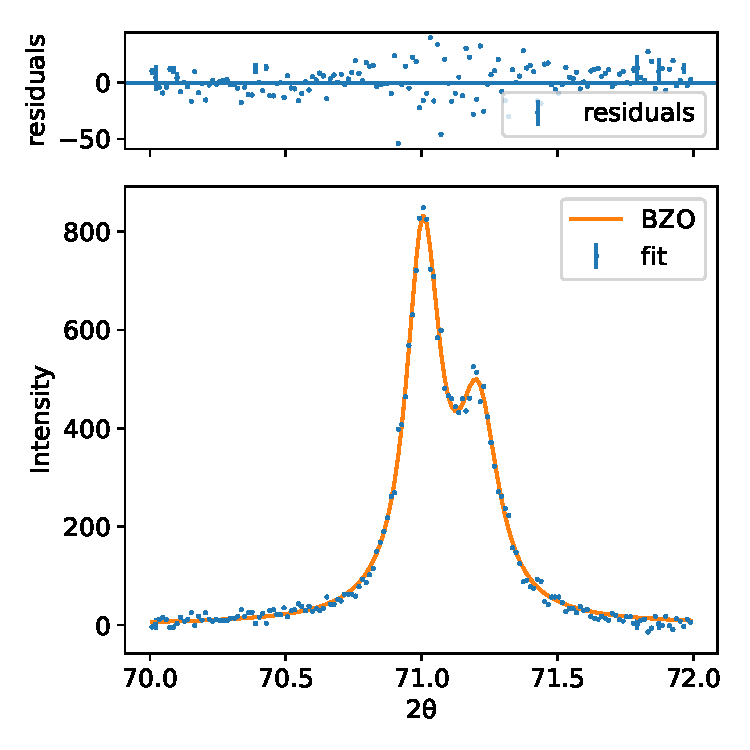
\includegraphics{Figures/190219-xrd-BZO-model-fit.pdf}
    \caption{Comparison of Pseudo-Voigt model fit with 310 peak on BZO XRD pattern.}
    \label{fig:target:xrd:fitComparison}
\end{figure}

When considering the uncertainty of each peak location ($\delta\theta$) extracted from fitting a model curve to the diffraction data and its effect of the uncertainty of the lattice parameter ($\delta a$) we can see the following relationship from the general principle of propagation of uncertainty \cite{Taylor1997},
\begin{equation}
\delta a = a \sqrt{\left(\frac{\partial a}{\partial \theta}\delta \theta\right)^2} = a \delta \theta \cdot \cot{\theta}.
\end{equation}Since the error in lattice constant is proportional to the cotangent, this error decreases as $\theta$ approaches 90\textdegree, or 180\textdegree\ in $2\theta$. Therefore a weighted average of lattice parameters should have larger weight applied to larger angles. Table \ref{tab:xrd:latticeParameterCalculation} shows the experimental peak fits for barium zirconate powder in which the weighted average for lattice parameter is $a = 4.19507 \pm 0.00004$\AA. It should be noted that this is the uncertainty from the model fitting and not of the total experimental uncertainty given uncertainties in detector positioning and alignment, which should be in the 0.0001 \AA\ range \cite{Herbstein2000}.

\begin{table}[tb]
    \centering
    \caption{Determination of lattice parameters for BZO powder at different diffraction angles. By calculating a weighted average the indices with high uncertainty are property handled. Uncertainty generally decreases with increasing diffraction angle.}
    \begin{tabular}{rrrr}
        \toprule
         (hkl) &    2 $\theta$ &         $a$ ($\mbox{\AA}$) &       $\delta a$  \\
        \midrule \midrule
         100 &  21.122494 &  4.206093 &  0.003 \\
         110 &  30.106436 &  4.197836 &  0.0001 \\
         111 &  37.112942 &  4.195815 &  0.0002 \\
         200 &  43.120790 &  4.195691 &  0.0001 \\
         210 &  47.235369 &  4.302777 &  0.004 \\
         211 &  53.508297 &  4.194837 &  0.00006 \\
         220 &  62.645205 &  4.194412 &  0.00007 \\
         310 &  71.070671 &  4.194498 &  0.00008 \\
        \bottomrule
        \end{tabular}
    \label{tab:xrd:latticeParameterCalculation}
\end{table}

Based on extracting the lattice parameter from these patterns, Table \ref{tab:target:xrd:latticeConstant} shows that with increasing dopant ion radius, the lattice parameter increases. This trend is important since one of the major concerns discussed in Chapter \ref{ch:background} with doping this material with a trivalent ion is that the dopant could substitute for the B site ion (Zr) and produce the desired oxygen vacancies to promote conduction of protons, or the dopant could substitute for the A site ions (Ba) and consume an oxygen vacancy. Since the ionic radius of barium is 149 pm, by putting any of these dopants in its place, a decrease of the lattice constant would be expected according to a Vegard's Law like approach where the lattice parameter would be the weighted average of the two constituent unit cells \cite{Denton1991}. However the substitution must predominantly be in the place of Zr since the lattice constant shows an expansion of the unit cell. 

\begin{table}[b]
    \centering
    \caption{Comparison of Dopant Radii and Lattice Parameters after heat treatment at 1600\textdegree C}
    \begin{tabular}{lrr}
        \toprule
        Dopant &  Radius &  Lattice Parameter \\
        \midrule
        \midrule
          pure &    72.0 &          4.194600 \\
            Yb &    86.8 &          4.200000 \\
             Y &    90.0 &          4.201100 \\
            Gd &    93.8 &          4.214645 \\
        \bottomrule
        \end{tabular}
    \label{tab:target:xrd:latticeConstant}
\end{table}

An important trend resulting from this analysis is shown in Figure \ref{fig:bulk:xrd:latticeParamDopantRadius} where the measured lattice parameters are plotted for the various dopants after the initial reaction step of heating at 1300\textdegree C as well as the final heat treatment at 1600\textdegree C. For each dopant there is a slight change in lattice parameter from the processing step at 1300\textdegree C and the treatment at 1600\textdegree C. In the case of ytterbium (Yb), the lattice parameter decreases after the high temperature process, while for both yttrium (Y) and gadolinium (Gd), the lattice parameter increases. All samples were made with the same dopant concentration and thus it is expected that the change in lattice parameter should depend only on dopant ionic radius. This can be understood in the context of Figure \ref{fig:target:xrd:reaction:dopants} and the ensuing discussion, which identified secondary phases of BaY\textsubscript{2}O\textsubscript{4} or BaGd\textsubscript{2}O\textsubscript{4} in the respective samples. With these two samples, the presence of the secondary phases following the 1300\textdegree C step means that some significant amount of the dopant is not incorporated into the barium zirconate structure and thus the lattice parameter of that structure is lower than would be expected for the concentration of dopant in the precursor powder mixture. This could arise from regions of the powder mixture that have a high concentration of dopant, possibly due to the grain size of the powders originally mixed together. This dry mixture of powders may need finer processing to produce smaller particles and thus a more homogeneous reaction and dopant incorporation. In addition to this possible difference in concentration affecting the lattice parameter measurement, the difference in thermal expansion coefficients between the primary and secondary phase may also be partially responsible for the lattice parameter distortion. The thermal expansion coefficient of the secondary BaY\textsubscript{2}O\textsubscript{4} phase is much higher than that of barium zirconate ($1.08\times 10^{-5}$ K$^{-1}$ vs. $7\times 10^{-6}$ K$^{-1}$ \cite{Maekawa2007, Zhao1991, Goretta1998, Yamanaka2005}). Thus the lattice of barium zirconate would be under compressive stress, yielding a reduced value for its lattice parameter as measured from the XRD peaks. 

After the higher 1600\textdegree C heat treatment and longer treatment time, the lattice parameter of the Yb-doped sample decreases while that of Y- and Gd-doped increases. The decrease in lattice parameter of the Yb-doped sample may be the result of BaO loss as it tends to evaporate at higher temperature. This can drive the Yb ions to Ba sites and result in a decrease in lattice parameter. In the case of the of Y- and Gd- doped samples, in both cases the secondary phases have decreased (and even disappeared in the Gd-doped case). This suggests that the dopants have incorporated into the lattice, and that due to the increase in lattice parameter that they have largely substituted for zirconium. 
\begin{figure}
    \centering
    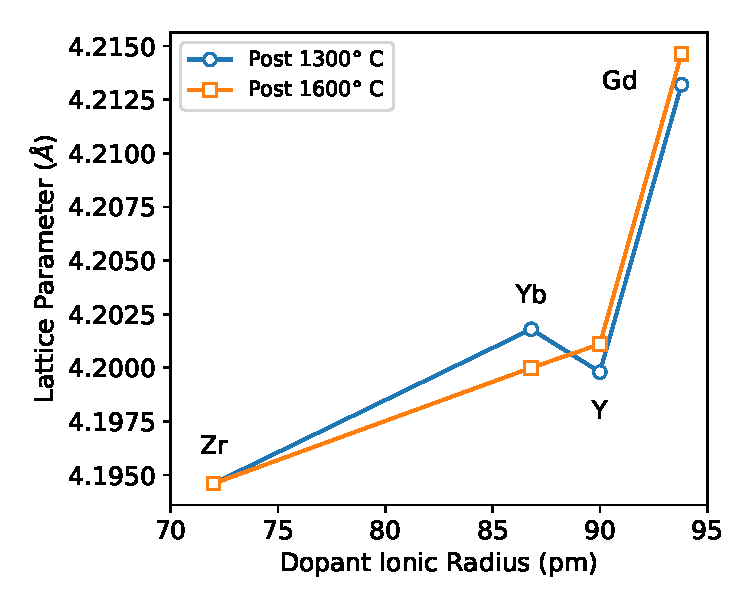
\includegraphics{Figures/190614-pellet-dopant-latticeParam-radius.pdf}
    \caption{Lattice parameters measured by XRD of bulk samples doped with elements of various ionic radius. Lines are a guide to the eye for change in lattice parameter with dopant radius following the indicated heat treatment.}
    \label{fig:bulk:xrd:latticeParamDopantRadius}
\end{figure}

Another feature is the much higher lattice constant of the gadolinium doped samples in comparison to the difference in ionic radius. This feature may stand out more due to the ytterbium and yttrium samples having lattice parameters lower than would be expected given the dopant levels of the samples. For the ytterbium case, the lack of any secondary phase, as indicated in Figure \ref{fig:target:xrd:reaction:dopants}, could suggest it is already at or beyond optimal stoichiometric ratio and further heat treatment reduces lattice parameter. But for yttrium, while the sample following 1300\textdegree C reaction shows secondary phase and thus a lowered lattice parameter, it also has this secondary phase following the 1600\textdegree C though diminished in relative intensity. Thus not only does the lattice parameter increase, but it is still lower than it could be expected if further heating was applied. 

It should be noted here that this case of having excess barium relative to dopant ions in the form of BaGd\textsubscript{2}O\textsubscript{4} in the bulk sample may in fact be the ideal due to the consideration of it serving as a future laser ablation target. Since the plasma plume generated during ablation is in effect another heating process, it represents an opportunity for further barium loss. Heating the target to 1600\textdegree C is necessary to sinter the material to be suitable in the vacuum environment and ablation process of PLD, but the deleterious effects on barium content could possibly be mitigated by the inclusion of excess barium carbonate to force the presence of this secondary phase. If future studies of barium content in PLD produced thin films show a deficiency, this would be a possible avenue of improvement to pursue.
\begin{figure}
    \centering
    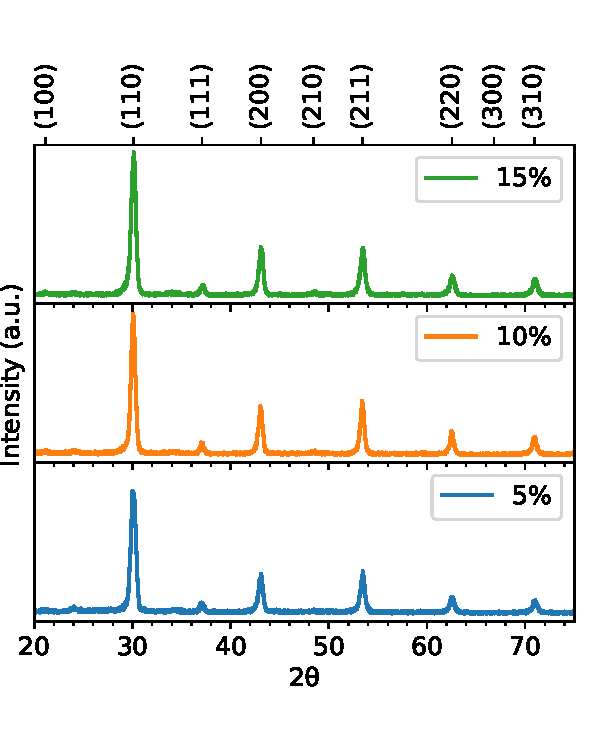
\includegraphics{Figures/150407-xrd-1stgen-dopant-concentration.pdf}
    \caption{2$\theta$ XRD scans of Gd-doped BaZrO$_3$ bulk samples produced without compensation for barium loss. All reflections of the BaZrO$_3$ crystal are noted to be present with relative intensities consistent with a randomly oriented polycrystal.}
    \label{fig:target:xrd:bariumCompensationComparison}
\end{figure}
To further support this idea of dopant placement, targets were made without compensating for the need for extra barium to incorporate the dopant ions with the correct stoichiometry. This was done by simply mixing barium zirconate powder with the desired amount of gadolinium oxide to achieve a dopant concentration with respect to zirconium content, but without additional barium oxide to force these ions to B sites. Concentration of 5\%, 10\%, and 15\% of Gd were mixed and heated to 1400\textdegree C, and then XRD was performed in order to determine the lattice parameters from the patterns using the above procedure. The corresponding 2$\theta$ XRD patterns for these samples without compensation for barium loss are shown in Figure \ref{fig:target:xrd:bariumCompensationComparison}.
\begin{table}[tb]
\caption{Lattice parameter and dopant concentration in targets uncompensated for barium loss.}
\centering
\label{tab:target:xrd:latticeParamVsDopantConcentration}
\begin{tabular}{ll}
\toprule
concentration & lattice parameter \\
\midrule \midrule
pure          & 4.1945            \\
5\%           & 4.1999            \\
10\%          & 4.2025            \\
15\%          & 4.1982            \\
\bottomrule
\end{tabular}
\end{table}
By extracting lattice parameters from this series of targets uncompensated for barium loss, Table \ref{tab:target:xrd:latticeParamVsDopantConcentration} summarizes the findings. Of note here is that the lattice parameter does increase by adding dopant to the targets, but that increasing the dopant level produces no clear trend in increasing the lattice parameter, as would be expected \cite{Fabbri2010c}. 



